\section{Discusión}
Los datos presentados aquí sugieren que la respuesta al SARS-CoV-2 está desequilibrada con respecto al control de la replicación del virus frente a la activación de la respuesta inmunitaria adaptativa.

\begin{figure}[h]
	\fbox{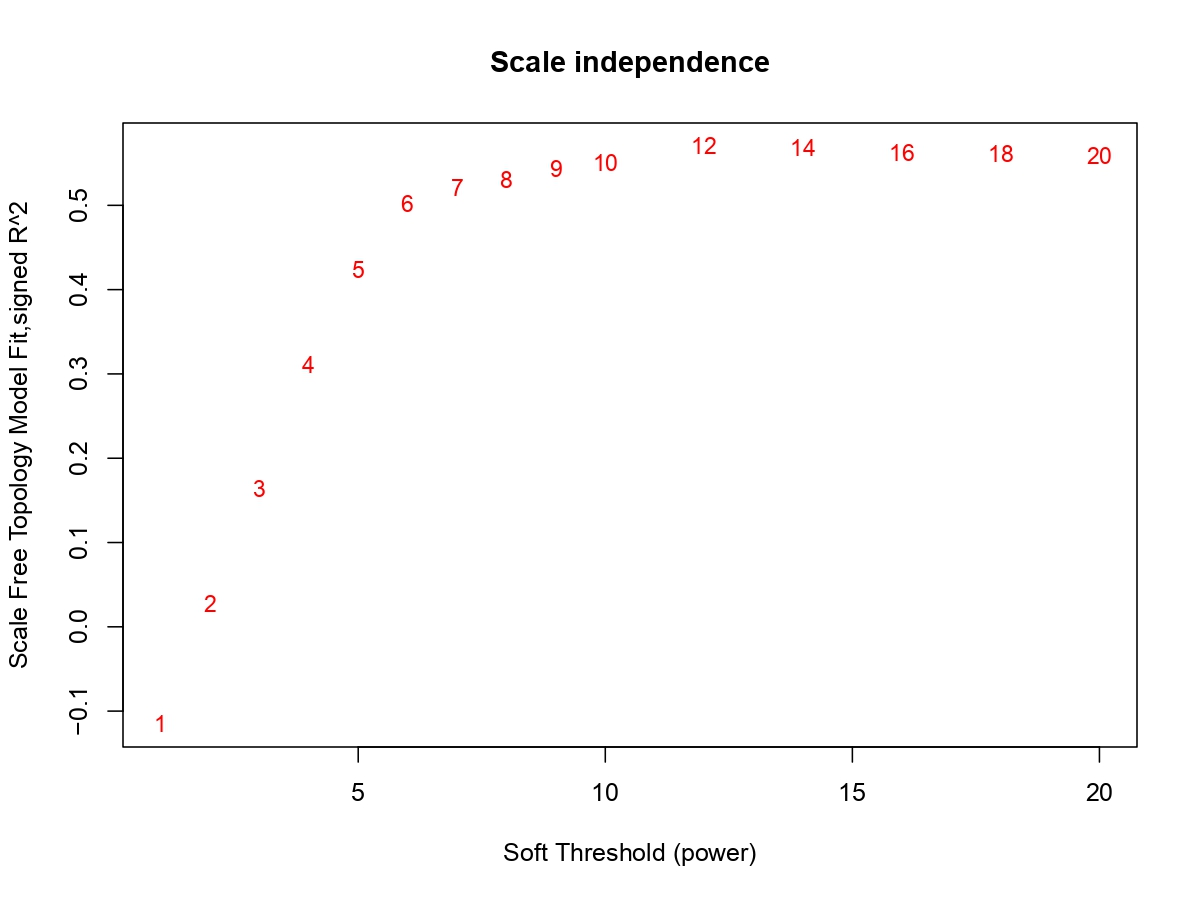
\includegraphics[width=0.9\textwidth]{figures/independenceScale_meanConnectivity1.jpg}}
	\caption{Independence Scale_mean Connectivity 1}
	\label{fig:sample_clustering}
\end{figure}

Dada esta dinámica, los tratamientos para la COVID-19 tienen menos que ver con la respuesta del IFN y más con el control de la inflamación. 

\begin{figure}[!]
	\fbox{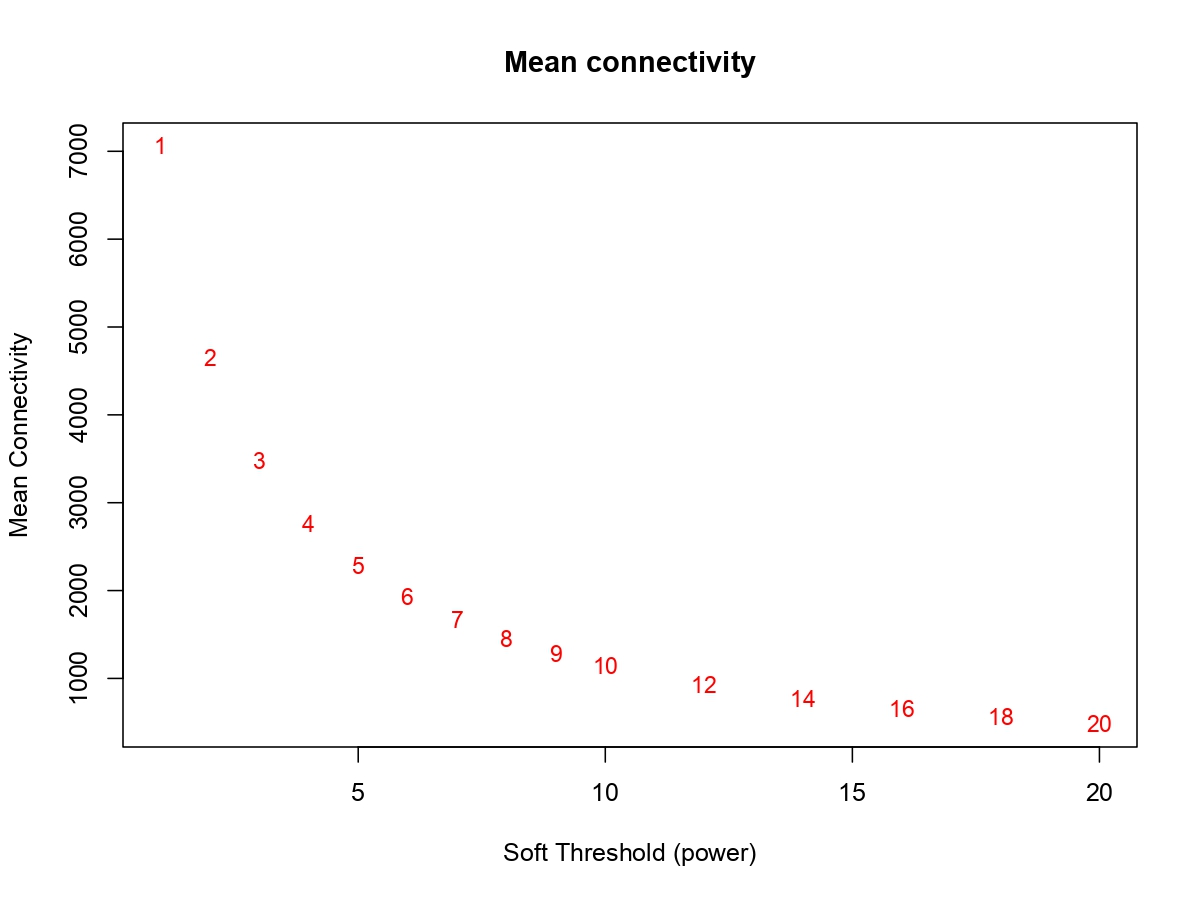
\includegraphics[width=0.9\textwidth]{figures/independenceScale_meanConnectivity2.jpg}}
	\caption{Independence Scale_mean Connectivity 2}
	\label{fig:sample_clustering}
\end{figure}
	
